\documentclass[12pt, a4paper, twoside]{article}

\usepackage{graphicx}
\usepackage[a4paper, left=2cm, right=2cm, top=2.5cm, bottom=3cm]{geometry}
\usepackage[utf8]{inputenc}
\usepackage[T1]{fontenc}
\usepackage{tcolorbox}
\usepackage{adjustbox}
\usepackage{geometry}
\usepackage{xparse}
\usepackage{float}
\usepackage{listings}
\usepackage{tabularx}
\usepackage{hyperref}

%Listingkonfiguration
\lstset{
  basicstyle=\ttfamily\small,
  breaklines=true,
  frame=none,
  language=MATLAB
}

\tcbuselibrary{listings, skins, breakable}

%Template für Codeerklärungsbox
\newtcolorbox{CodeErklaerungBox}[2][]{
  enhanced,
  breakable,
  colback=white,
  colframe=gray,
  fonttitle=\bfseries,
  title=#2,
  sidebyside,
  sidebyside align=center,
  lefthand width=0.47\textwidth,
  righthand width=0.47\textwidth,
  #1
}



\setlength{\fboxsep}{0.5pt}
\setlength{\fboxrule}{1pt}

\begin{document}
    \thispagestyle{empty}
     \vspace*{4cm}
    \begin{center}
        \includegraphics[width=200pt]{Bilder/Helmut Schmidt Universität-a89973ff.png}\\
        \vspace{2cm}
        \huge\textbf{MATLAB - Grundlagen für Ingenieurwissenschaften}
    \end{center}
    \newpage

    \pagenumbering{arabic}
    \renewcommand{\contentsname}{Inhaltsverzeichnis}
    \tableofcontents
    \newpage
    \section{Einführung}
        \subsection{Was ist MATLAB?}
        MATLAB ist die Abkürzung für MATrix LABoratory. Zudem ist es ein interaktives, integriertes System zur Berechnung, Visualisierung oder Programmierung mathematischer Problemstellungen. Es bietet eine einfache Skriptsprache welche auf die Verarbeitung von Matrizen ausgelegt ist.
        \subsection{Anwendungsgebiete in den Ingenieurwissenschaften}
        MATLAB bietet in vielen Ingenieurwissenschaftlichen Betätigungsfeldern weitreichende \\Vorteile.
        \begin{itemize}
            \item Signalverarbeitung
            \item Regelungstechnik
            \item FEM-Simulation
            \item Schaltungsanalyse
            \item Bildverarbeitung
            \item Datenanalyse
        \end{itemize}
        \subsection{Die Benutzeroberfläche}
            \subsubsection*{Command Window}
                \begin{figure}[H]
                    \centering
                    \fbox{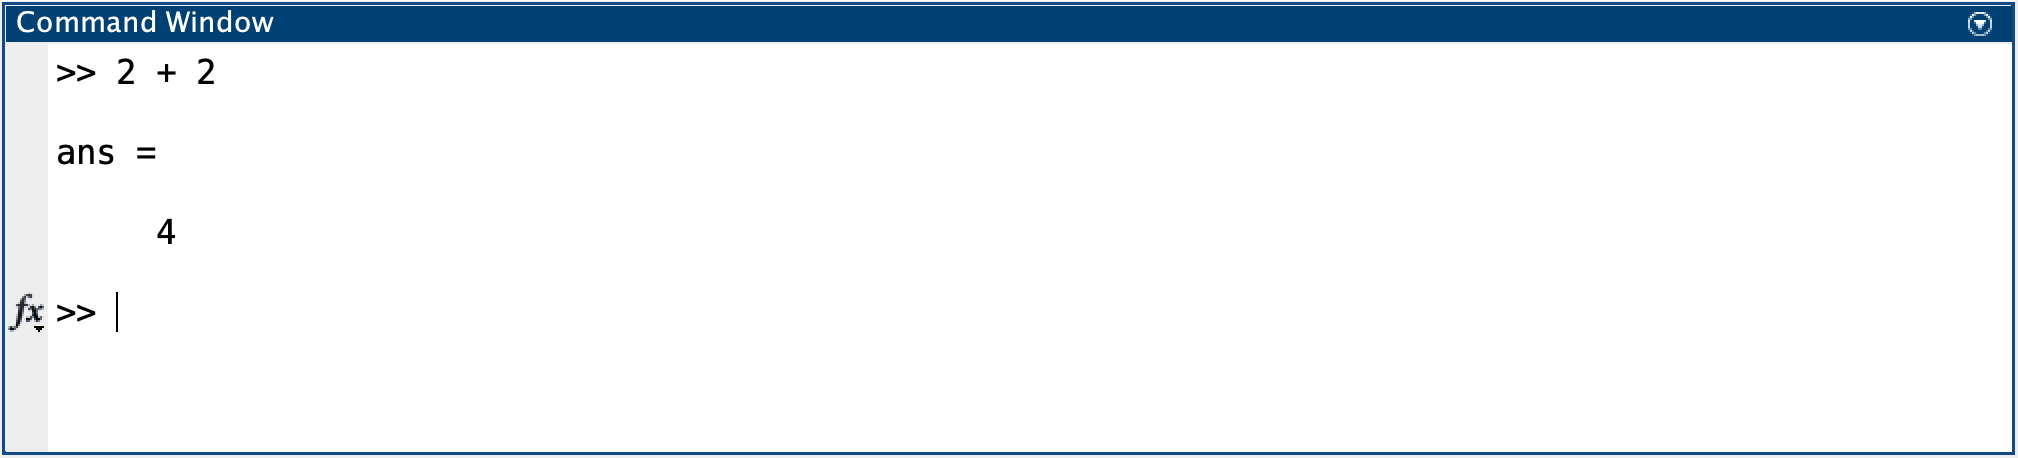
\includegraphics[width=0.7\textwidth]{Bilder/CommandWindow.png}}
                    \caption{Command Window in MATLAB}
                \end{figure}
                Im Command Window können Befehle direkt eingegeben werden. Da Ergebnisse von Berechnungen unverzüglich angezeigt werden, können hier einzelne Befehle idealerweise getestet werden.
            \subsubsection*{Editor}
                \begin{figure}[H]
                    \centering
                    \fbox{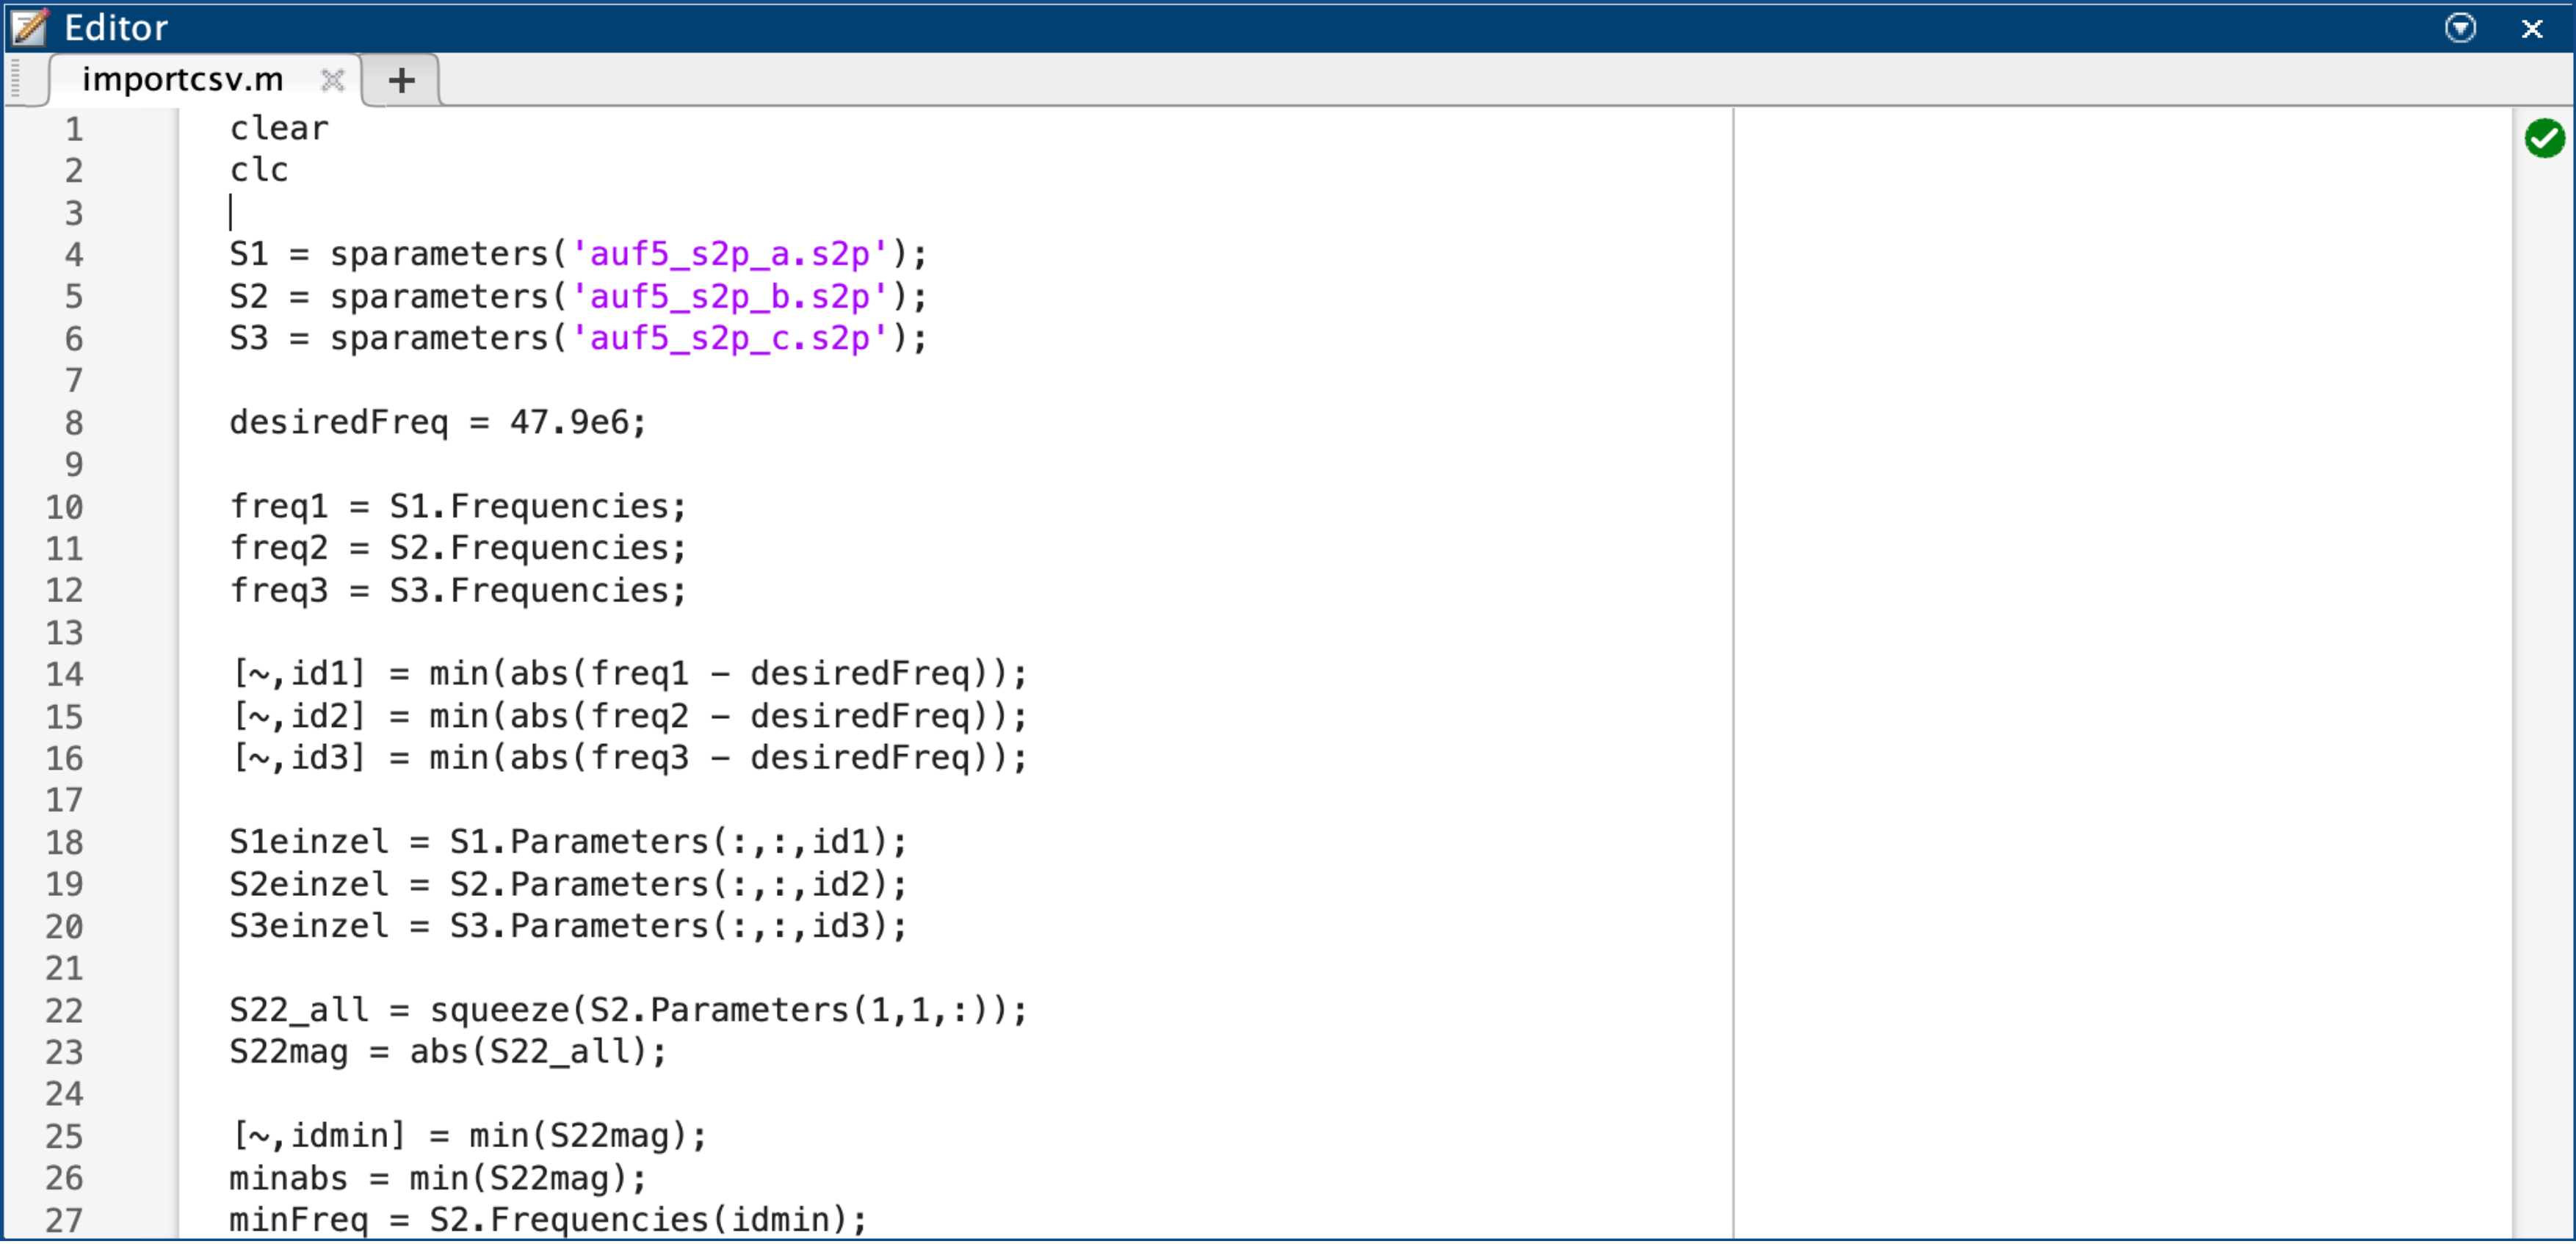
\includegraphics[width=0.7\textwidth]{Bilder/Editor.png}}
                    \caption{Editor in MATLAB}
                \end{figure}
                Im Editor können komplette Skripte und Funktionen geschrieben, gespeichert und ausgeführt werden. Er unterstützt das Debugging mittels Breakpoints und Schritt-für-Schritt Ausführung.
            \subsubsection*{Workspace}
                \begin{figure}[H]
                    \centering
                    \fbox{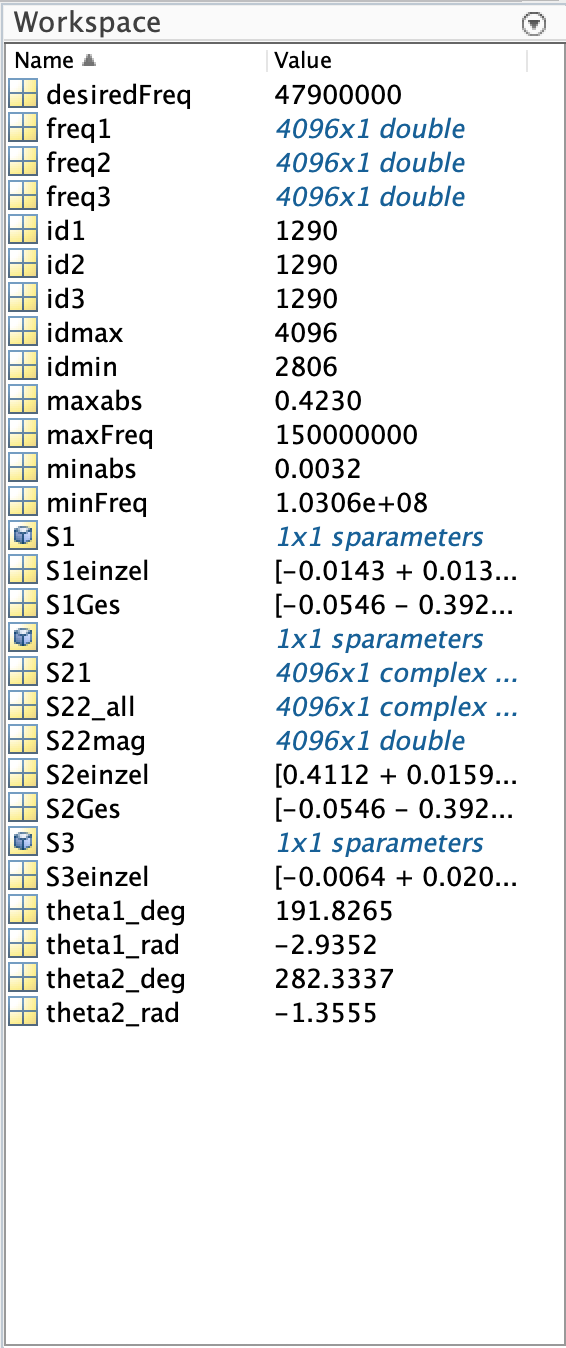
\includegraphics[width=0.2\textwidth]{Bilder/Workspace.png}}
                    \caption{Workspace in MATLAB}
                \end{figure}
                Im Workspace werden alle aktuellen Variablen inklusive ihres Inhalts angezeigt. Weiterhin ist es möglich diese Variablen hier manuell anzupassen oder zu löschen.
            \subsubsection*{Current Folder}
                \begin{figure}[H]
                    \centering
                    \fbox{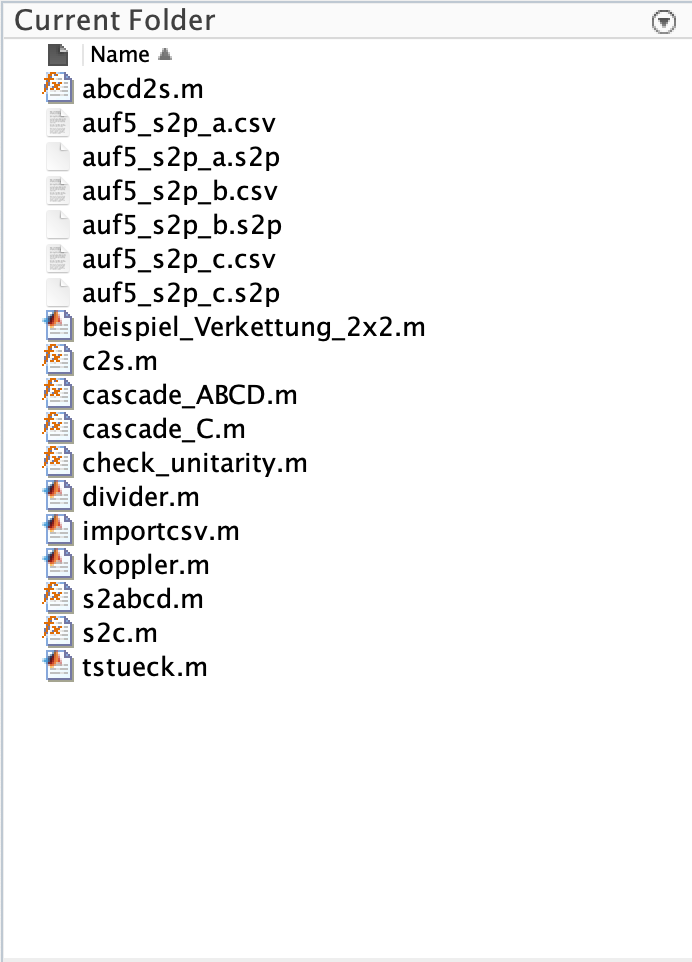
\includegraphics[width=0.3\textwidth]{Bilder/CurrentFolder.png}}
                    \caption{Current Folder in MATLAB}              
                \end{figure}
                Im Current Folder findet man alle Dateien des Projektordners. Diese können durch Doppelklick oder das Ziehen in den Editor geöffnet und bearbeitet werden.
            \newpage
            
    \section{Grundlegende Operationen}
        \subsection{Variablendeklaration}
                \begin{CodeErklaerungBox}{Einfache Wertzuweisung}
                \begin{lstlisting}
a = 3;
                \end{lstlisting}
                \tcblower
                Der Variable \texttt{a} wird der Wert \texttt{3} zugewiesen.
                \end{CodeErklaerungBox}
                \noindent Eine Zuweisung ohne ein Semikolon am Ende der Zeile bewirkt eine direkte Rückgabe des Variablenwertes.
                \begin{CodeErklaerungBox}{Fließkommazahl}
                \begin{lstlisting}
a = 4.5;
                \end{lstlisting}
                \tcblower
                Der Variable \texttt{a} wird der Wert \texttt{4.5} zugewiesen. Als Trennzeichen in MATLAB wird der Punkt an Stelle eines Kommas verwendet.
                \end{CodeErklaerungBox}
                \begin{CodeErklaerungBox}{Zeichenkette}
                \begin{lstlisting}
name = "Peter";
                \end{lstlisting}
                \tcblower
                Der Variable \texttt{name} wird der String \texttt{Peter} zugewiesen.
                \end{CodeErklaerungBox}
                \begin{CodeErklaerungBox}{Logischer Wert}
                \begin{lstlisting}
isValid = true;
                \end{lstlisting}
                \tcblower
                Der Variable \texttt{isValid} wird der boolsche Wert \texttt{true} zugewiesen.
                \end{CodeErklaerungBox}
                \begin{CodeErklaerungBox}{Automatische Typzuweisung}
                \begin{lstlisting}
a = pi;
                \end{lstlisting}
                \tcblower
                Der Variable \texttt{a} wird die, in MATLAB vordefinierte Variable $\pi$ zugewiesen.
                \end{CodeErklaerungBox}
                \noindent Neben pi gibt es weitere vordefinierte Variablen. Diesen kann zwar ebenfalls ein selbst definierter Wert zugewiesen werden, jedoch ist es nicht empfehlenswert.
                \begin{center}
                \renewcommand{\arraystretch}{1.4}
                \begin{tabularx}{\textwidth}{|l| X| l|}
                    \hline
                    \textbf{Variable} & \textbf{Bedeutung} & \textbf{Wert} \\
                    \hline
                    \texttt{inf} & Unendlich & $\frac{1}{0}$ ergibt \texttt{inf} \\
                    \hline
                    \texttt{i} & Imaginäre Einheit & $\sqrt{-1}$ \\
                    \hline
                    \texttt{j} & Alternative imaginäre Einheit & $\sqrt{-1}$ \\
                    \hline
                    \texttt{NaN} & "Not a Number" - ungültiger Wert & $\frac{0}{0}$ ergibt \texttt{NaN} \\
                    \hline
                    \texttt{ans} & Ergebnis der letzten berechneten Zeile & z.B. \texttt{ans = 42} \\
                    \hline
                    \texttt{true}/\texttt{false} & Boolsche Werte & \texttt{1} bzw. \texttt{0} \\
                    \hline
                \end{tabularx}
            \end{center}
        \subsection{Mathematische Grundoperationen}
        \subsection{Kommentare}
        \subsection{Komplexe Zahlen}
    \section{Vektoren und Matrizen}
        \subsection{Erstellen von Vektoren und Matrizen}
        \subsection{Zugriff auf Elemente und Indizierung}
        \subsection{Matrixoperationen}
        \subsection{nuetzliche MATLAB Funktionen}
    \section{Programmiergrundlagen}
        \subsection{Skripte}
        \subsection{Funktionen}
        \subsection{Schleifen}
    \section{Arbeiten mit Dateien und Daten}
        \subsection{Speichern und Laden von Daten}
        \subsection{Importieren von Messdaten}
        \subsection{Analyse und Verarbeitung von Daten}
    \section{Visualisierung von Daten}
        \subsection{Einfache Diagramme}
        \subsection{Mehrere Kurven in einem Diagramm}
        \subsection{Mehrere Diagramme in einer UEbersicht}
        \subsection{Grafische Anpassungen}
    \section{Anhang}
        \subsection{Dokumentation in MATLAB}
        \subsection{Uebersicht wichtiger MATLAB Befehle}
\end{document}
